\documentclass[8pt]{article}
\usepackage{graphicx}
	\setkeys{Gin}{width=0.4\textwidth}
\usepackage[a4paper]{geometry}
\usepackage{listings}
\newcommand*{\deriv}{\ensuremath{\mathrm{d}}}
\twocolumn
\begin{document}
	\author{Jonathan Cancio \\ Oliver Atienza \\ Justin Balderas \\ 
	Reyster Fresco \\ Yna Ojeda \\ Ethan Tan \\ Marc Teves \\ Troy Valdez}
	\title{CS 131 MP2: Analysis of stock market prices as a function of previous price, volume, and momentum}
	\maketitle
	\section{Abstract}
	% Make sure to always have one sentence per line.
	Stock prices seem to be unpredictable.
	Predicting the future price of shares in a particular company will allow stock traders to make more profitable trading strategies.
	The group tried to predict the closing price of seven different companies on 24 May 2018. 
	The group performed a linear regression on their closing price, trading volume, and closing price momentum over varying timespans.
	The prediction error was found to be (to be continued...)
	\section{Introduction}

	Stock prices are unpredictable because there are simply too many factors that can influence the price of shares.
	While it would not be impossible to gather all the possible factors that could affect the price of a specific stock and make a mathematical equation describing how each factors into predicting the future price of a stock, it is likely that there are too many factors for any human built system to track.

	The most obvious way of making money in the stock market via trading stocks is \textit{arbitrage}, more commonly known as "buy low, sell high".
	Less known is the more effective technique called \textit{momentum investing}, summarized as "buy high, sell higher". 

	Momentum investing became a popular strategy after investors and economists noticed that if a stock has been performing well over a time period of three to twelve months, then it will continue to do well.
	That is, if the price of a stock has had high returns for a long time, then it will continue to have high returns.
	On the other hand, if a stock has had poor returns for a long time, then it will continue to have low returns.

	This tendency to stay increasing or decreasing is known as \textit{momentum}, and can be quantified as the derivative of stock price at a specific point in time.

	$$ m_{t} = \frac{\deriv P(t)}{\deriv t} $$

	where $P(t)$ is the price at time $t$.

	If momentum investing is a good strategy, then there is some function

	$$ P(t, m) $$

	that reasonably predicts $P(t)$ at some future $t$. If $$P(t,m)$$ was a 
	linear sum 

	$$ P(t,m) = \alpha f(t) + \beta m_{t} $$

	then it must be that $\beta > 0$, which indicates that the momentum 
	positively influences stock prices, so that it is consistent with 
	momentum investing theory.

	A good guess for $P(t,m)$, the \textit{predictor} would be 

	$$ P(t_{k+1},m) = \alpha P(t_{k}) + \beta V(t_{k}) + \gamma m_{t_k}$$

	This equation simply says that the current price is a linear sum of the previous price, the previous trading volume, and the momentum.

	In the real world, instead of a function $P(t)$, instead there are several data points that give the price $P$ for each point in time $t$.
	Thus, its derivative, the value for $m_{t}$, cannot be solved analytically, but it can be solved numerically.
	Instead of finding the exact value of the derivative, it is estimated.

	One way to estimate the derivative of a function is the \textit{centered difference formula}

	$$ m_{t} = \frac{\deriv P(t)}{\deriv t} = \frac{P(t+h) - P(t-h)}{2h} $$

	This equation uses two data points before and after the point of interest to obtain an approximation of $m_{t}$.

	With this equation, it is now possible to obtain the momentum without knowledge of $P(t)$, as long as $P(t+h)$ and $P(t-h)$ are known.

	On account of the inaccuracy incurred by solving for the derivative analytically, the predictor is modified:

	$$ P(t_{k+1},m) = \alpha P(t_{k}) + \beta V(t_{k}) +
	\gamma m^{h=22}_{t_k} + \sigma m^{h=7}_{t_k}$$

	\section{Methodology}

	\begin{figure}[h]
		\centering
		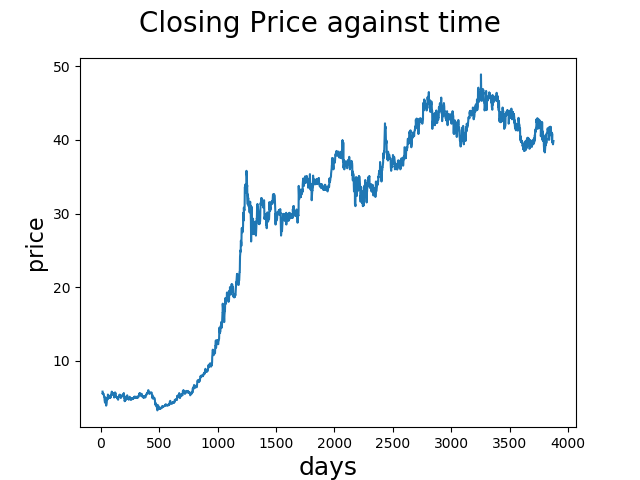
\includegraphics{ap_closing_price.png}
		\caption{Closing prices}
		\label{fig:close_price_graph}
	\end{figure}

	Take a look at Figure~\ref{fig:close_price_graph}. On the x-axis is
	\texttt{days} and the y-axis is \textbf{price}
	\subsection{Preprocessing}
	In this section we take a look at the data processing required to make the
	data workable.
		\subsubsection{Removing irrelevant companies}
		Go through each entry one by one and delete it if it's not one of the tracked companies.

	\section{Results}
	\section{Discussion}
	\section{Conclusion}
	\begin{thebibliography}{9}
		\bibitem{heath}
			Heath M.,

			\textit{Scientific Computing - An Introductory Survey}
	\end{thebibliography}
\end{document}
